\section{Optimal Transport with Linear Programming}

In this notebook, we are introduced to a linear program solver. Given two weighted point clouds of mass $1$ (ie. two discrete probability distributions), setting a cost matrix $C$, we can compute the optimal transport plan. 

\begin{figure}[h]
     \centering
     \begin{subfigure}[b]{0.49\textwidth}
         \centering
         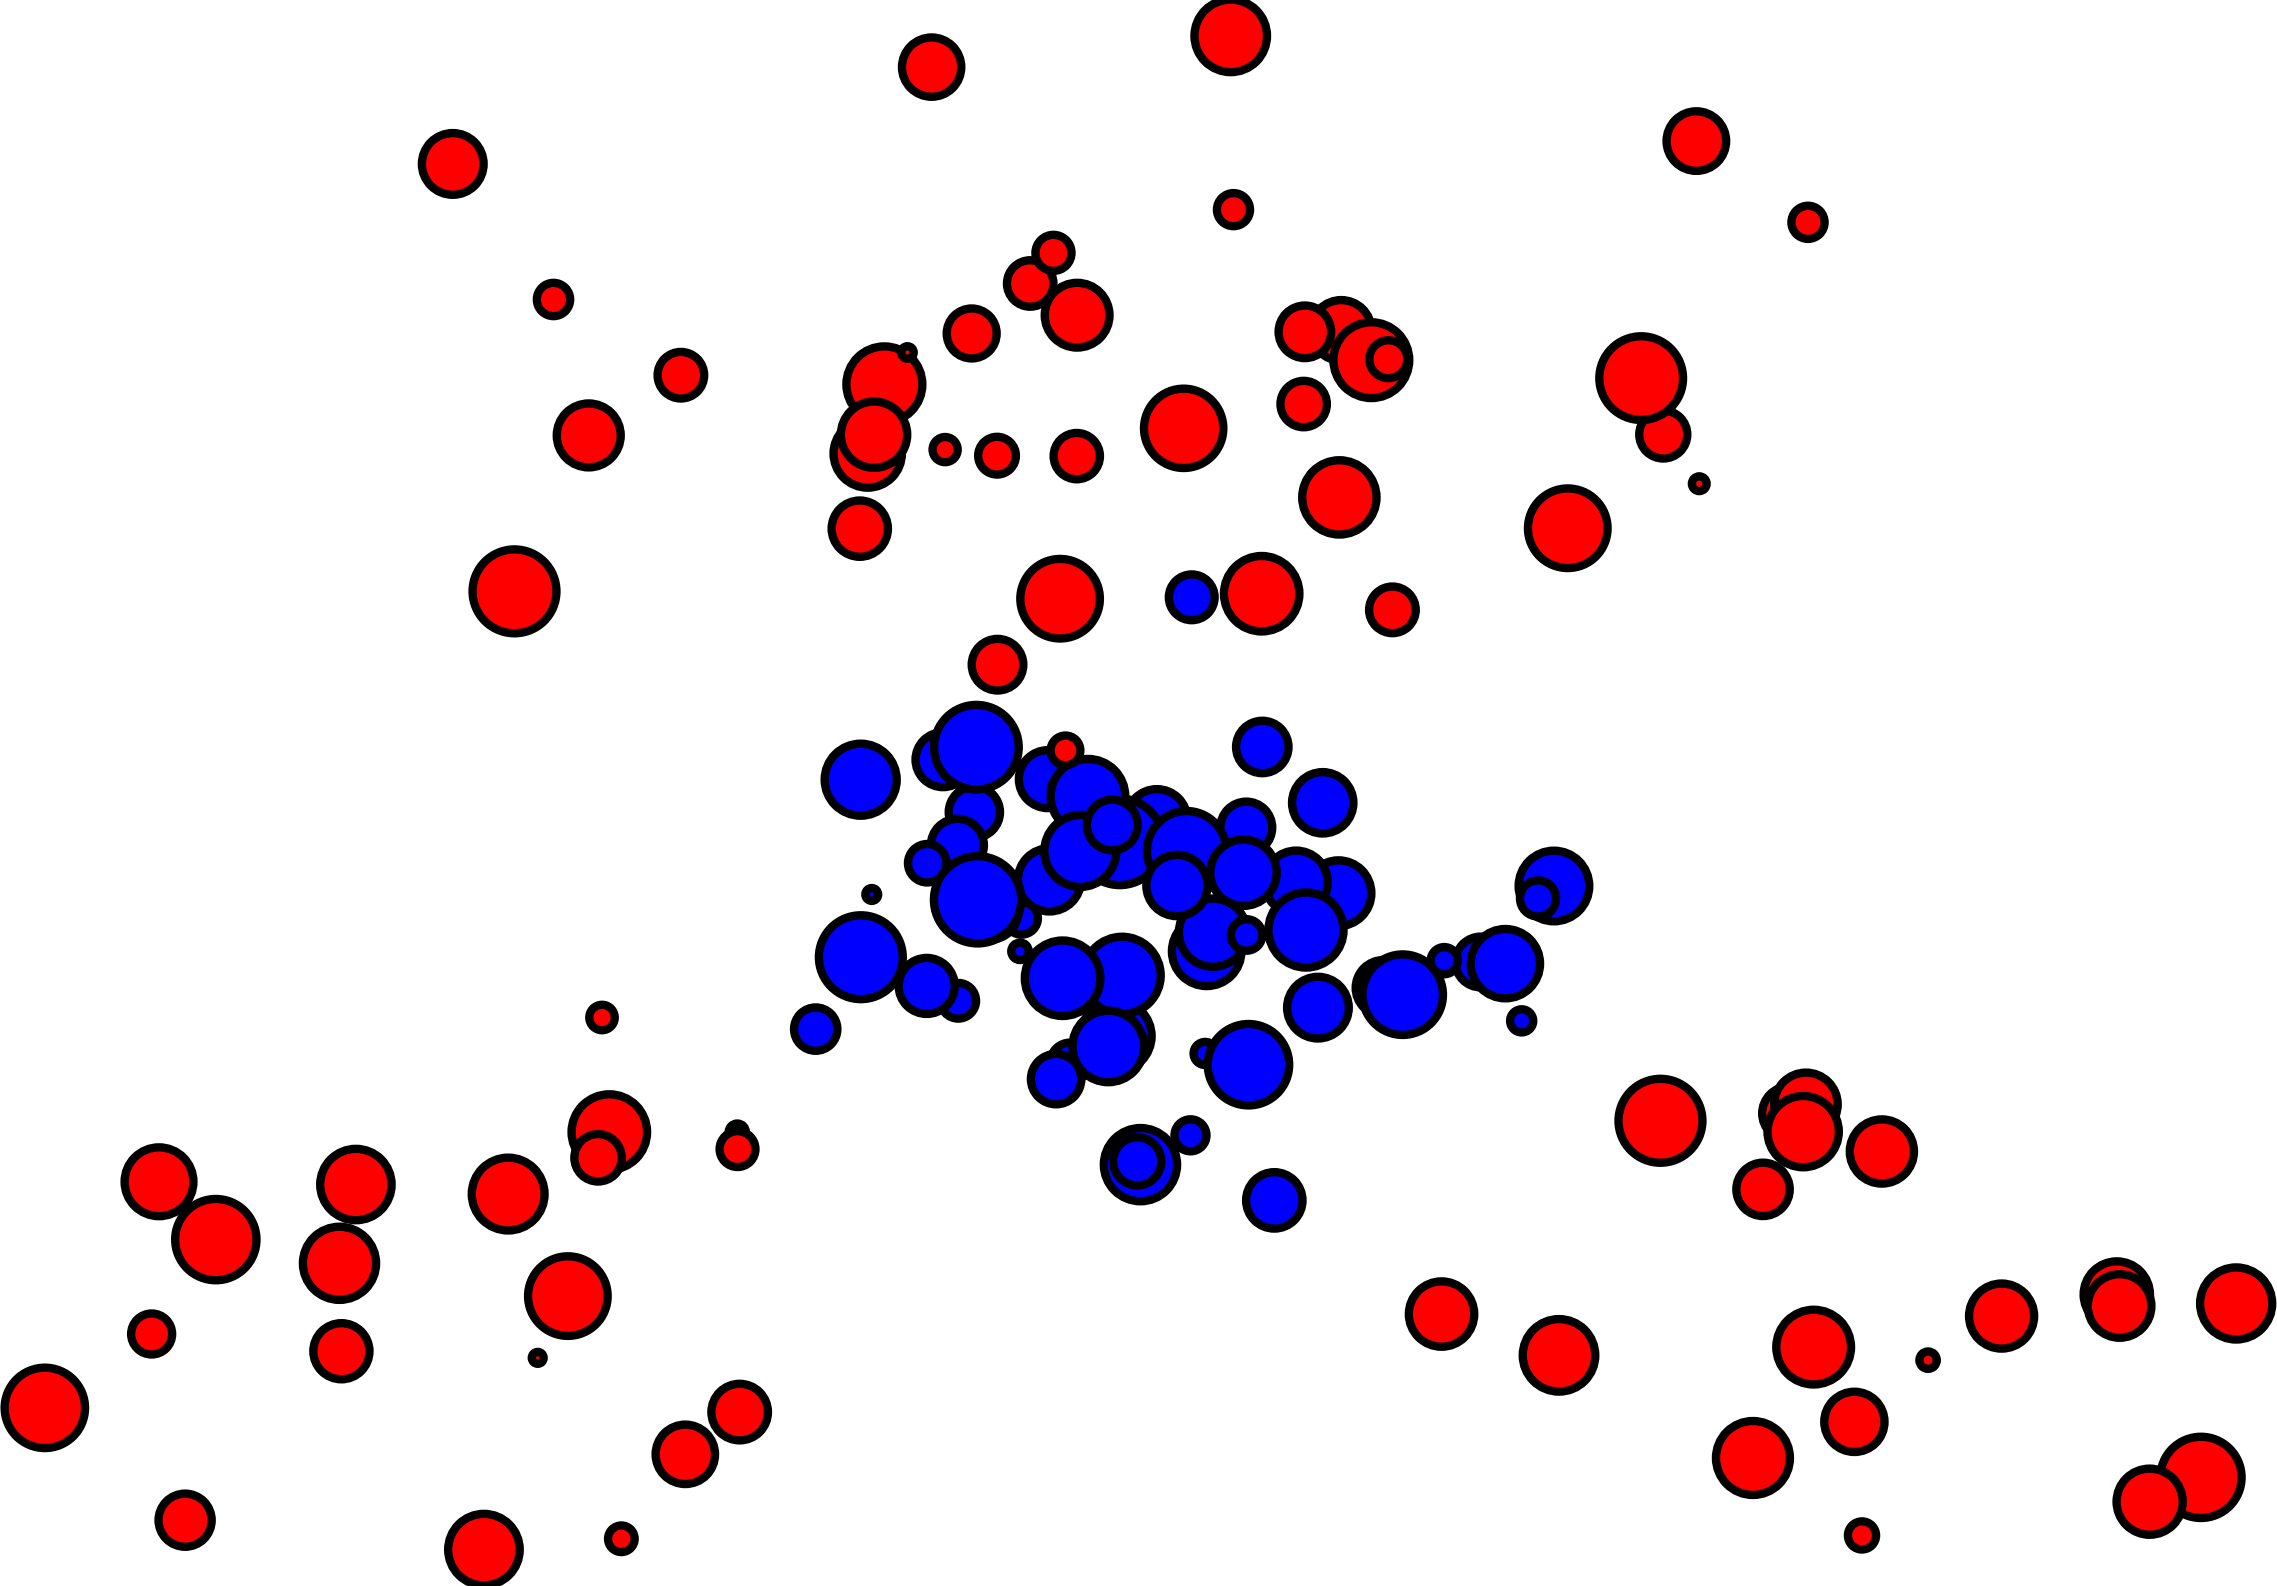
\includegraphics[width=\textwidth]{samples/1/point_cloud.png}
         \caption{Two distributions on $\RR^2$}
     \end{subfigure}
     \hfill
     \begin{subfigure}[b]{0.49\textwidth}
         \centering
         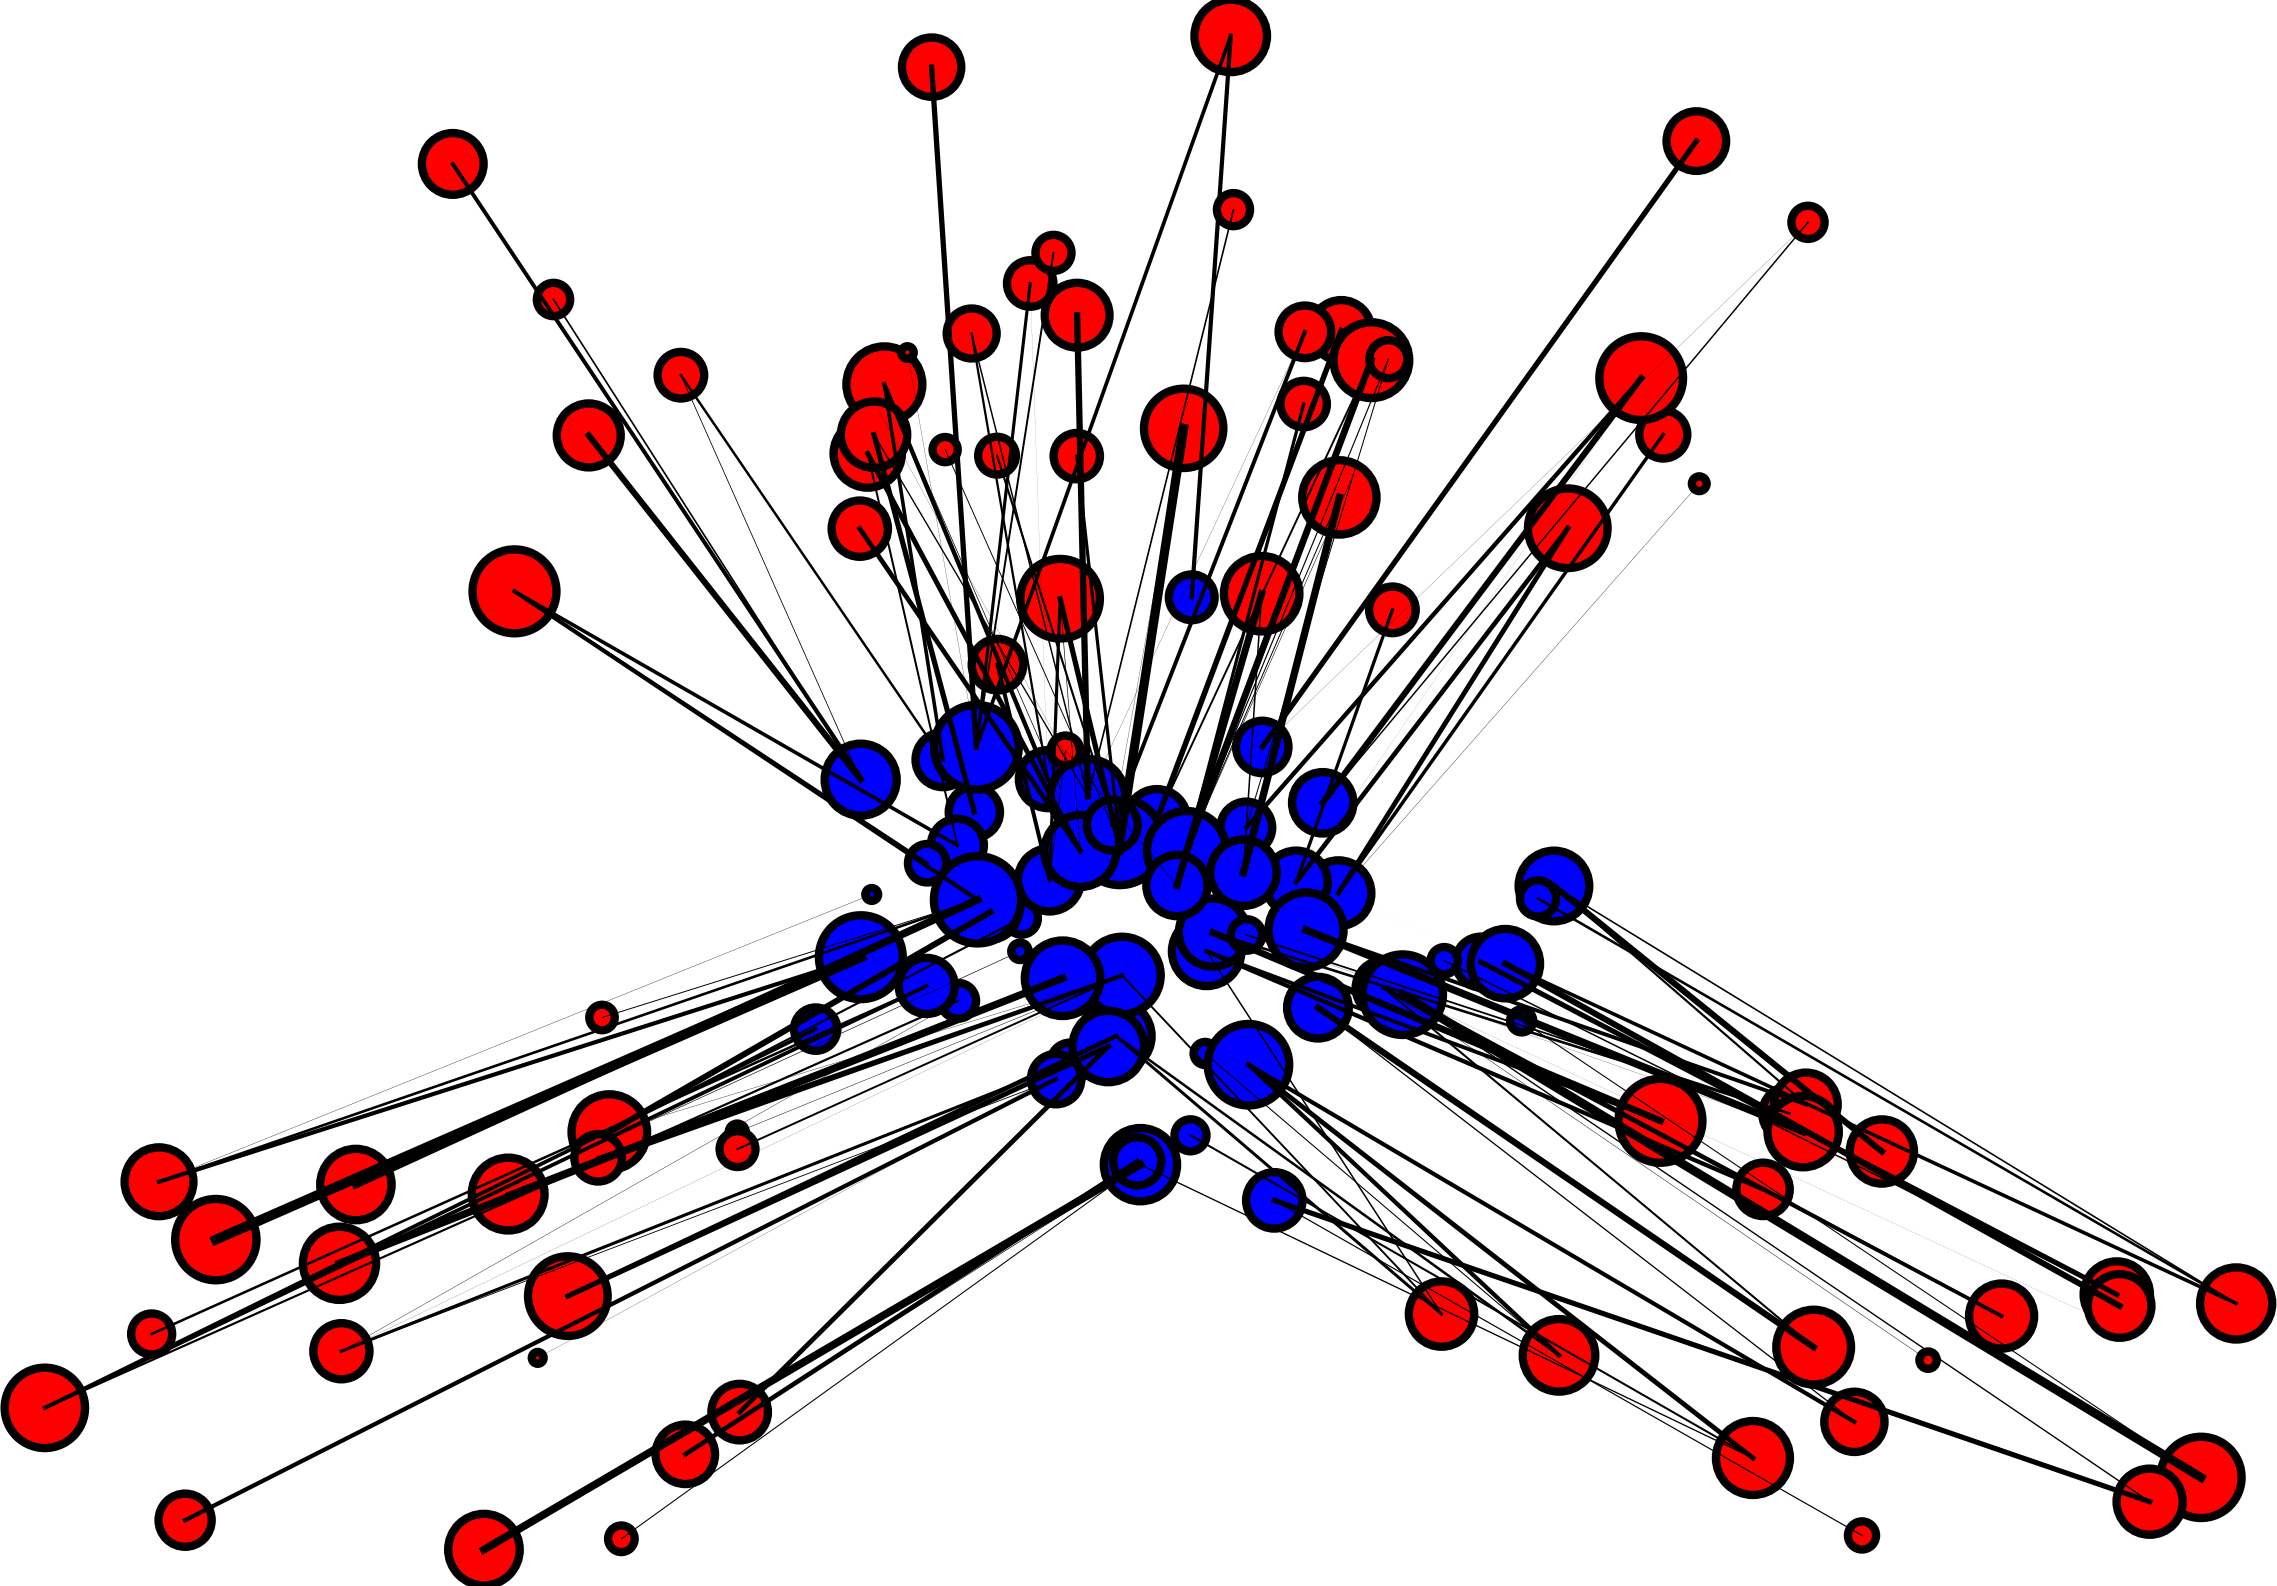
\includegraphics[width=\textwidth]{samples/1/point_cloud_OT.png}
         \caption{The optimal transport for $\LL_2$ norm}
     \end{subfigure}
    \caption{Two distributions and their optimal transport plan. Width of the lines are proportional to the quantity transported.}
\end{figure}

We have tools to check the validity of the solution: 
\begin{itemize}
    \item The coupling $P$ should have no more than $n+m-1$ non zero entries. Otherwise, the associated graph has at least one cycle, so $P$ is not an extremal point of the simplex, and thus can't be optimal.
    \item The solution must be feasible, ie. $P$ should meet: $P \one_m = a$ and $P^T \one_n = b$.
    \item If we had access to the dual variable, we would check that the complementary slackness is verified, but \texttt{perform\_linprog.py} only returns the primal solution.
\end{itemize}

Most of the content of the notebook was already given, so there is not much to comment; still, we can see the influence of the \textbf{cost matrix} on the coupling $P$. We use a basic distribution, as in fig. \ref{fig:easy_dist}.

\begin{figure}[p]
    \centering
    \begin{subfigure}[c]{0.4\textwidth}
    \centering
        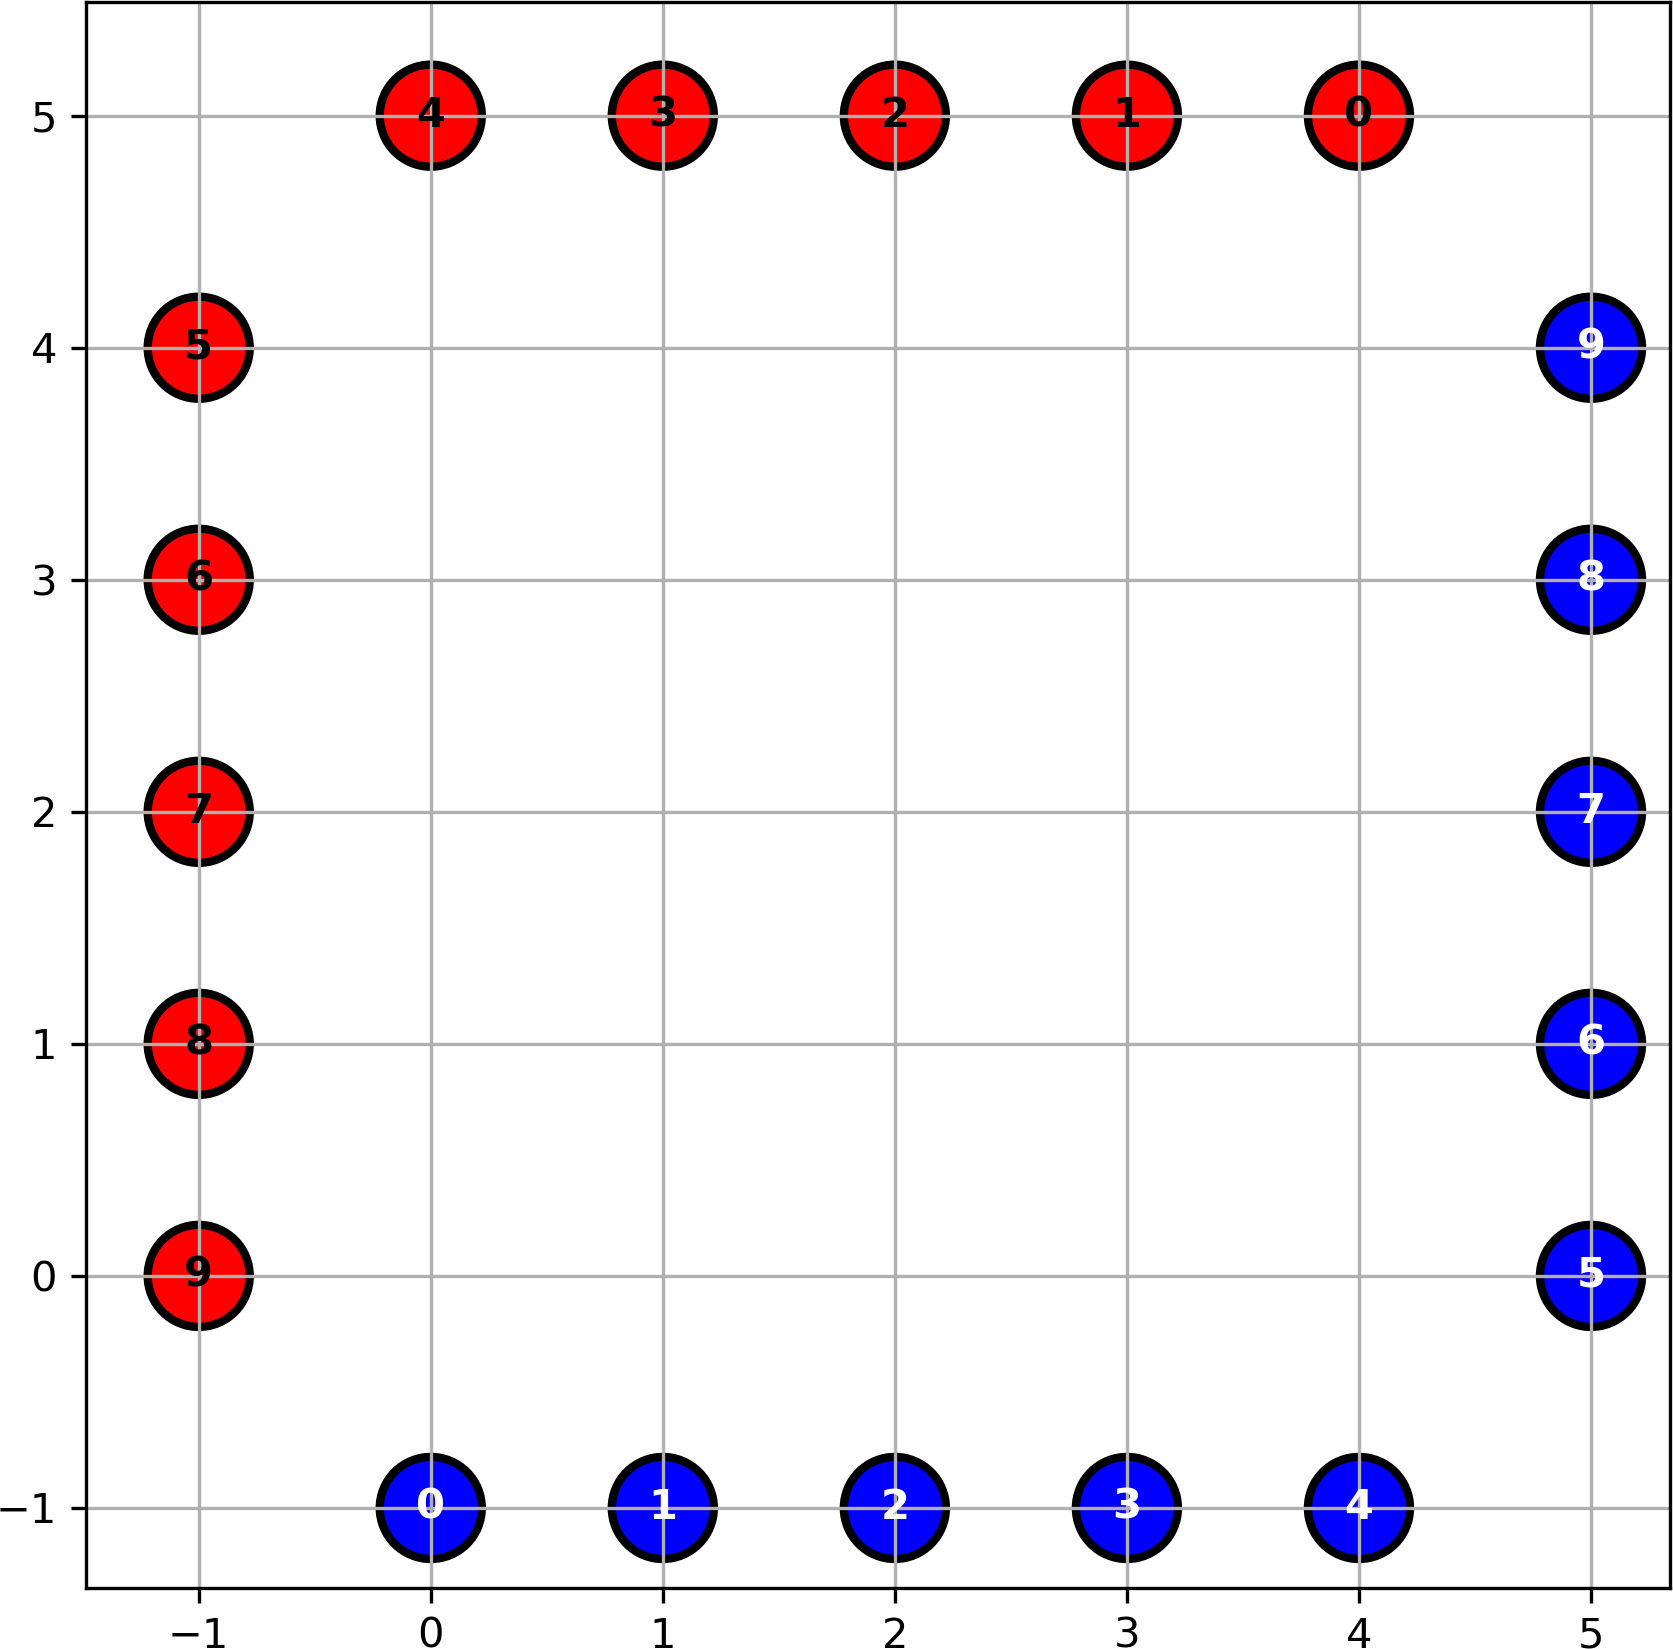
\includegraphics[width=\linewidth]{samples/1/easy_distributions.png}
        \caption{Two distributions on $\RR^2$.}
        \label{fig:easy_dist}
    \end{subfigure}
    \hfill
    \begin{subfigure}[c]{0.5\textwidth}
    \centering
        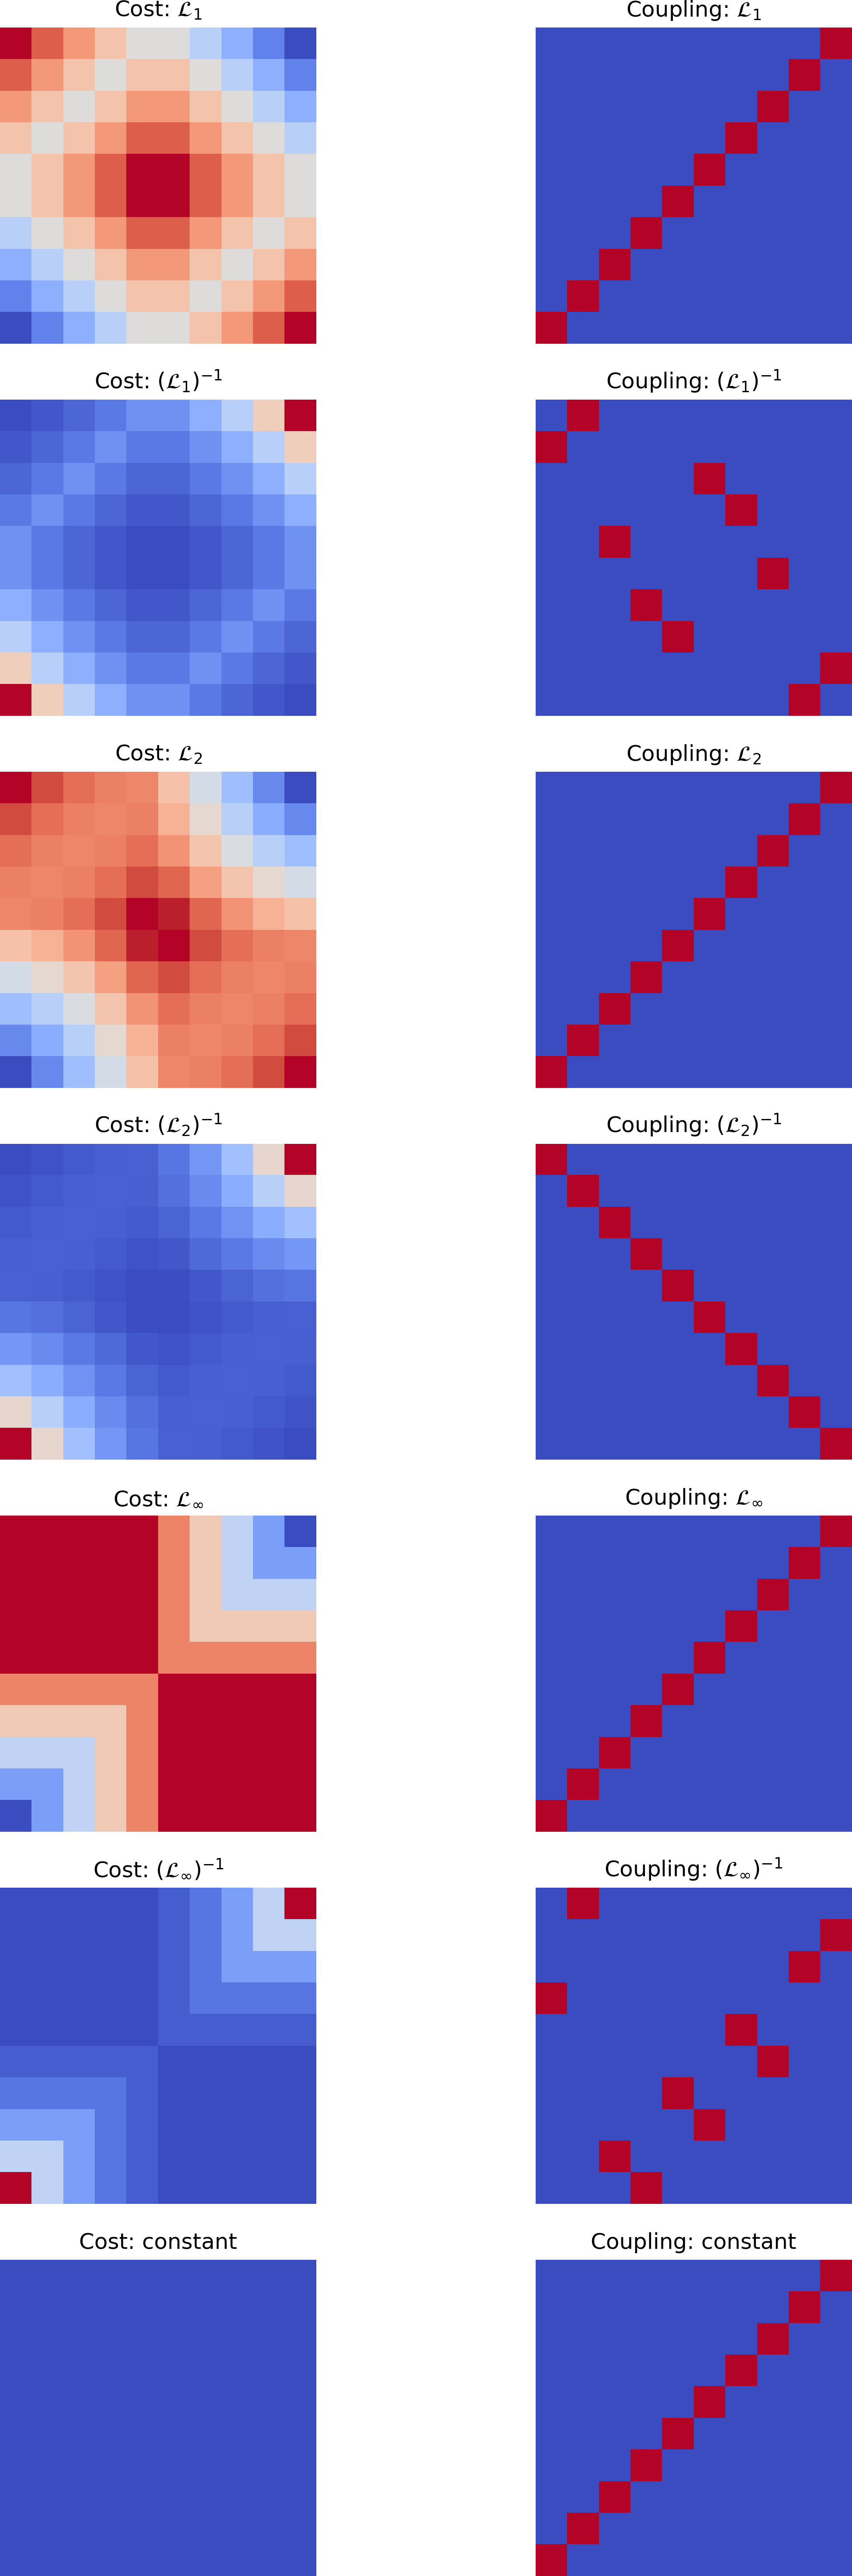
\includegraphics[width=\linewidth]{samples/1/all_couplings.png}
        \caption{Several cost and their associated optimal coupling.}
    \end{subfigure}
    \caption{Influence of the cost matrix $C$ on the optimal coupling. Here, the cost matrix is either a $\LL_p$ distance or an attractive metric, $1/||. ||_{\LL_p}$. For the inverse of the $\LL_{\infty}$ norm, the linear program did not converge.}
    \label{fig:comparaison_of_distances}
\end{figure}

I tried various cost matrix $C$: the ones associated with the $\LL_1$, $\LL_2$, $\LL_{\infty}$ norm, and a constant cost. For each of these cost (except for the constant one, obviously), I also looked at the \textbf{inverse} of the distance, to mimic an \textbf{attractive cost}. Here, by "inverse", I mean: 
\begin{equation*}
    C_{i, j}' = \frac{1}{C_{i, j}}
\end{equation*}

Of course, it is not a distance anymore, so the total cost has not the property of the Wassertein distance. Results are on fig. \ref{fig:comparaison_of_distances}.

Several comments:
\begin{itemize}
    \item All weights are uniform, so the optimal coupling will be a \textbf{permutation matrix.}
    \item I expected the behaviour to vary with the choice of $p$ for the $\LL_p$ norm. In fact, it does not, and what matters is only the relative order between the points.
    \item However, they are multiple behaviour for the cost matrix I fashioned by taking the inverse of the $\LL_p$ norms. 
    \item The solver reported an error for the attractive cost derived from the $\LL_{\infty}$ metric. Indeed, the output is not an optimum, as we can note that for instance: 
    \begin{equation*}
        1.66 \approx \sum \mathbb{I}_{ij} C_{ij} < \sum P^{\LL_\infty^{-1}}_{ij} C_{ij} \approx 2.48
    \end{equation*}
    where $\mathbb{I}$ is the identity matrix, and corresponds for example at the optimal coupling for $\LL_2^{-1}$ (fig. \ref{fig:comparaison_of_distances}, 4th row). 
    \item For the cost corresponding to the inverse of the $\LL_1$ norm, I was surprised that the optimal coupling \textbf{was not symetric}. In fact, they are \textbf{multiple minima}. For instance: 
    \begin{equation*}
        A = \left(
            \begin{matrix}
            0 & 1 & 0 & 0 & 0 & 0 & 0 & 0 & 0 & 0 \\
            1 & 0 & 0 & 0 & 0 & 0 & 0 & 0 & 0 & 0 \\
            0 & 0 & 0 & 0 & 0 & 1 & 0 & 0 & 0 & 0 \\
            0 & 0 & 0 & 0 & 0 & 0 & 1 & 0 & 0 & 0 \\
            0 & 0 & 1 & 0 & 0 & 0 & 0 & 0 & 0 & 0 \\
            0 & 0 & 0 & 0 & 0 & 0 & 0 & 1 & 0 & 0 \\
            0 & 0 & 0 & 1 & 0 & 0 & 0 & 0 & 0 & 0 \\
            0 & 0 & 0 & 0 & 1 & 0 & 0 & 0 & 0 & 0 \\
            0 & 0 & 0 & 0 & 0 & 0 & 0 & 0 & 0 & 1 \\
            0 & 0 & 0 & 0 & 0 & 0 & 0 & 0 & 1 & 0
            \end{matrix}
            \right) \quad
        B = A^T \quad
        C = \left(
            \begin{matrix}
            0 & 1 & 0 & 0 & 0 & 0 & 0 & 0 & 0 & 0 \\
            1 & 0 & 0 & 0 & 0 & 0 & 0 & 0 & 0 & 0 \\
            0 & 0 & 0 & 0 & 0 & 1 & 0 & 0 & 0 & 0 \\
            0 & 0 & 0 & 0 & 0 & 0 & 1 & 0 & 0 & 0 \\
            0 & 0 & 0 & 0 & 0 & 0 & 0 & \mathbf{1} & 0 & 0 \\
            0 & 0 & \mathbf{1} & 0 & 0 & 0 & 0 & 0 & 0 & 0 \\
            0 & 0 & 0 & 1 & 0 & 0 & 0 & 0 & 0 & 0 \\
            0 & 0 & 0 & 0 & 1 & 0 & 0 & 0 & 0 & 0 \\
            0 & 0 & 0 & 0 & 0 & 0 & 0 & 0 & 0 & 1 \\
            0 & 0 & 0 & 0 & 0 & 0 & 0 & 0 & 1 & 0
            \end{matrix}
            \right) \\
    \end{equation*}
    All these 3 matrices report a cost of $\approx 1.19$. 
\end{itemize}

Finally, some of the couplings of \ref{fig:comparaison_of_distances} are shown on fig. \ref{fig:some_couplings}.

\begin{figure}
    \centering
    \begin{subfigure}[c]{.5\textwidth}
        \centering
        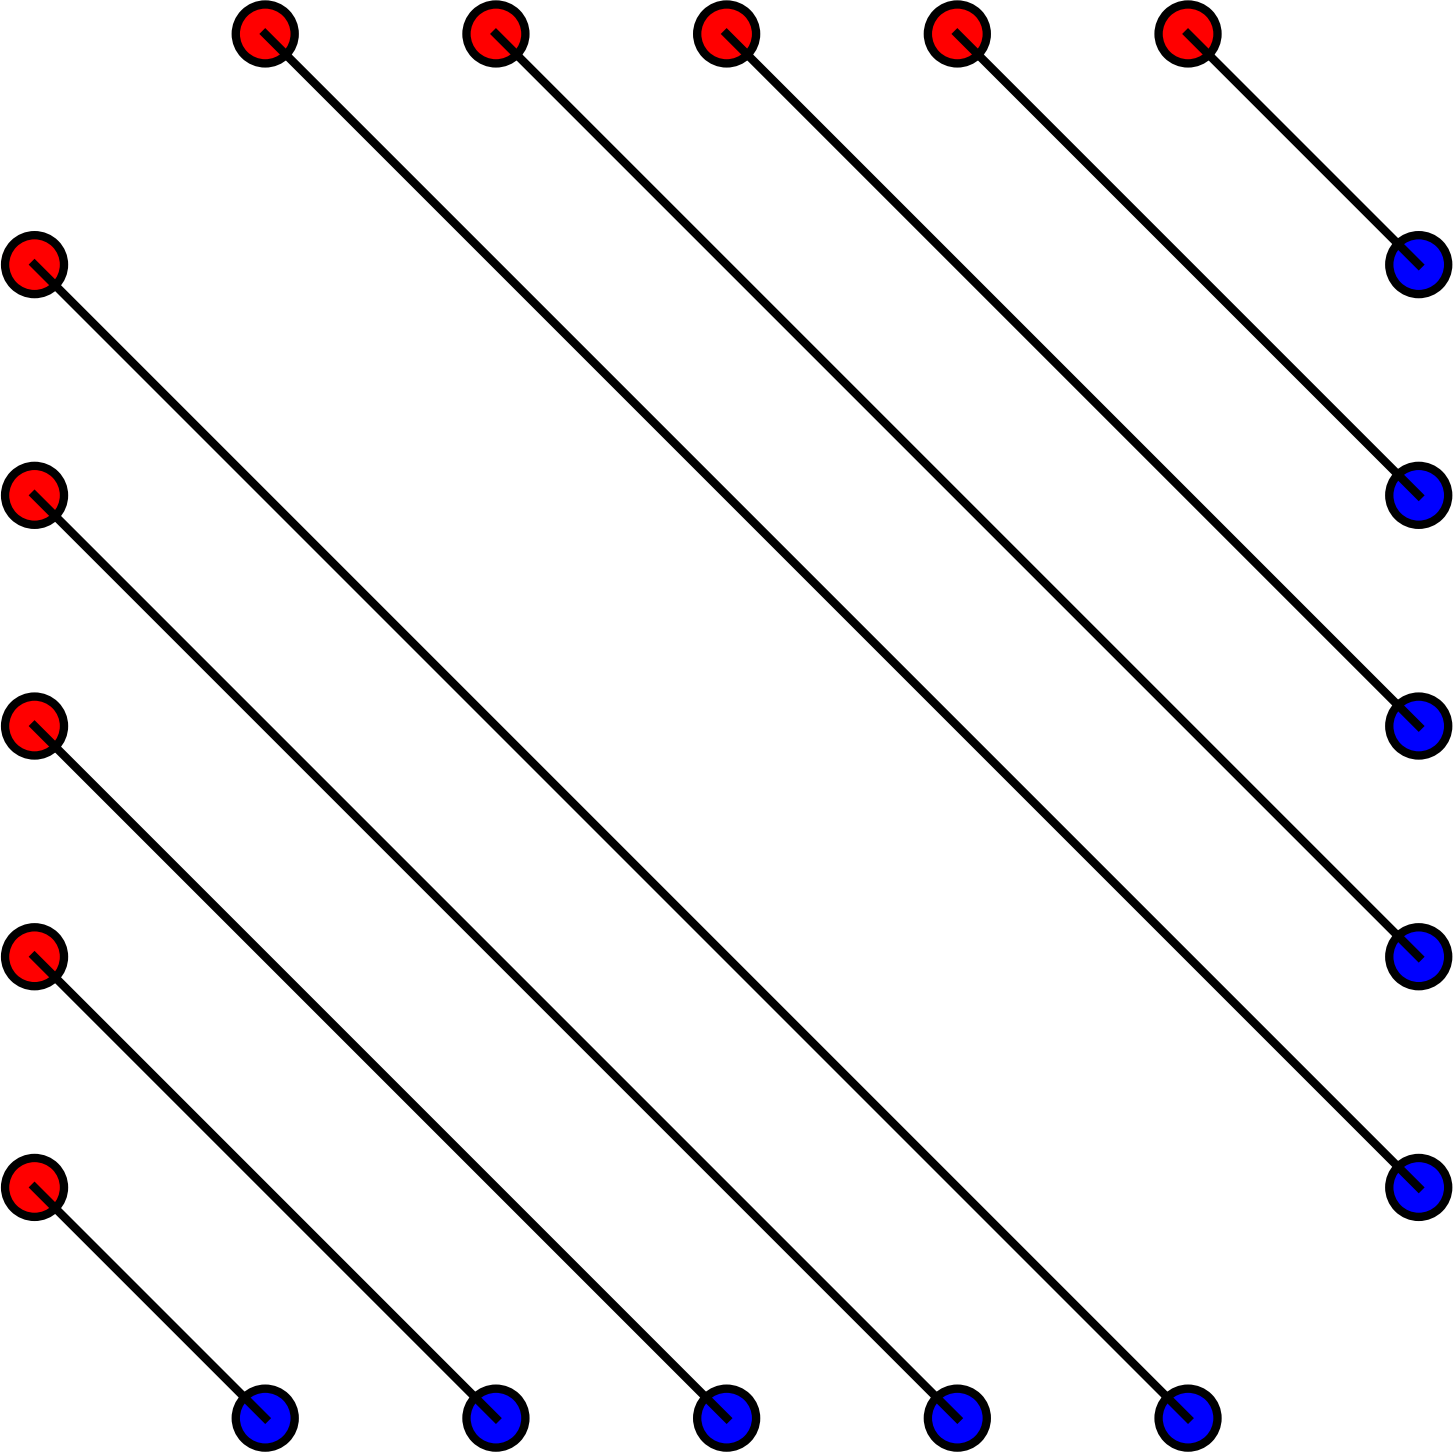
\includegraphics[width=\textwidth]{samples/1/l2_coupling.png}
        \caption{$\LL_2$ cost}
    \end{subfigure}
    
    \begin{subfigure}[c]{.5\textwidth}
        \centering
        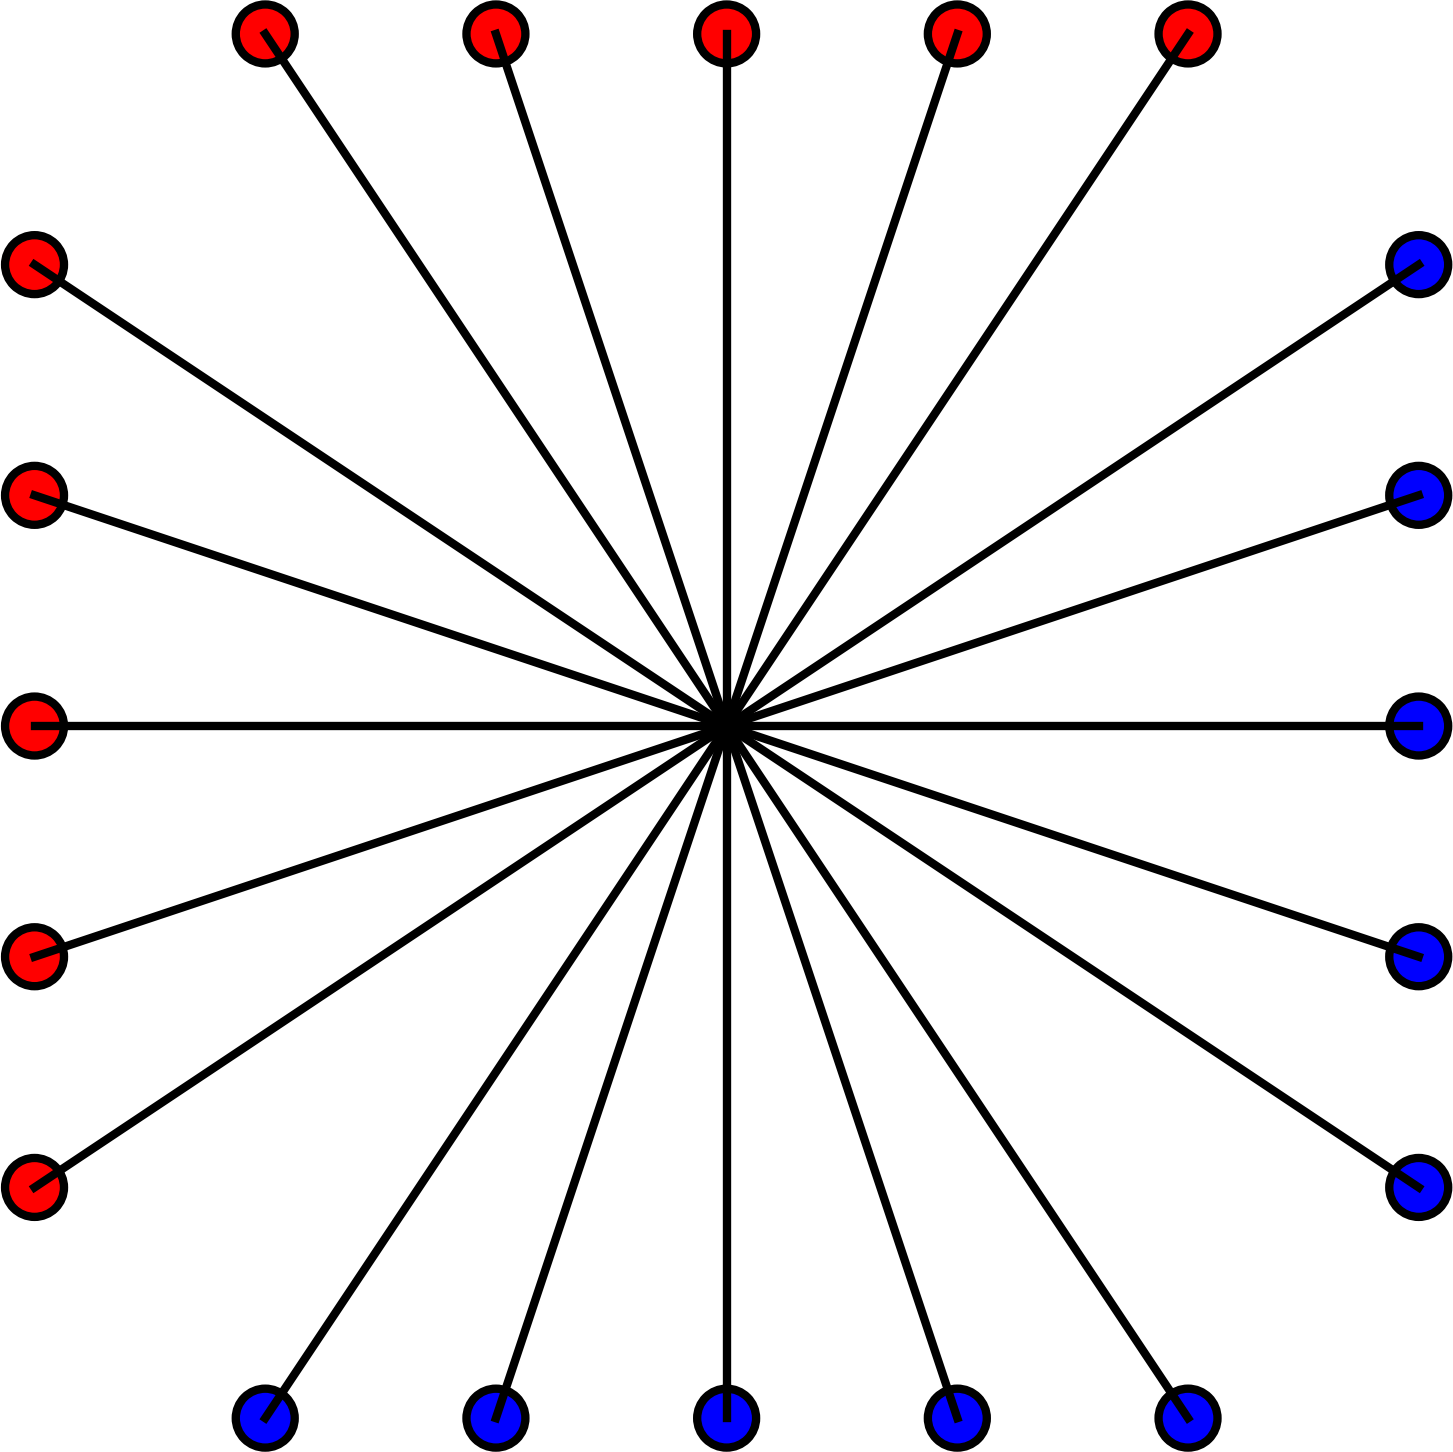
\includegraphics[width=\textwidth]{samples/1/l2_attract_coupling.png}
        \caption{$\LL_2^{-1}$, attractive cost}
    \end{subfigure}
    
    \begin{subfigure}[c]{.5\textwidth}
        \centering
        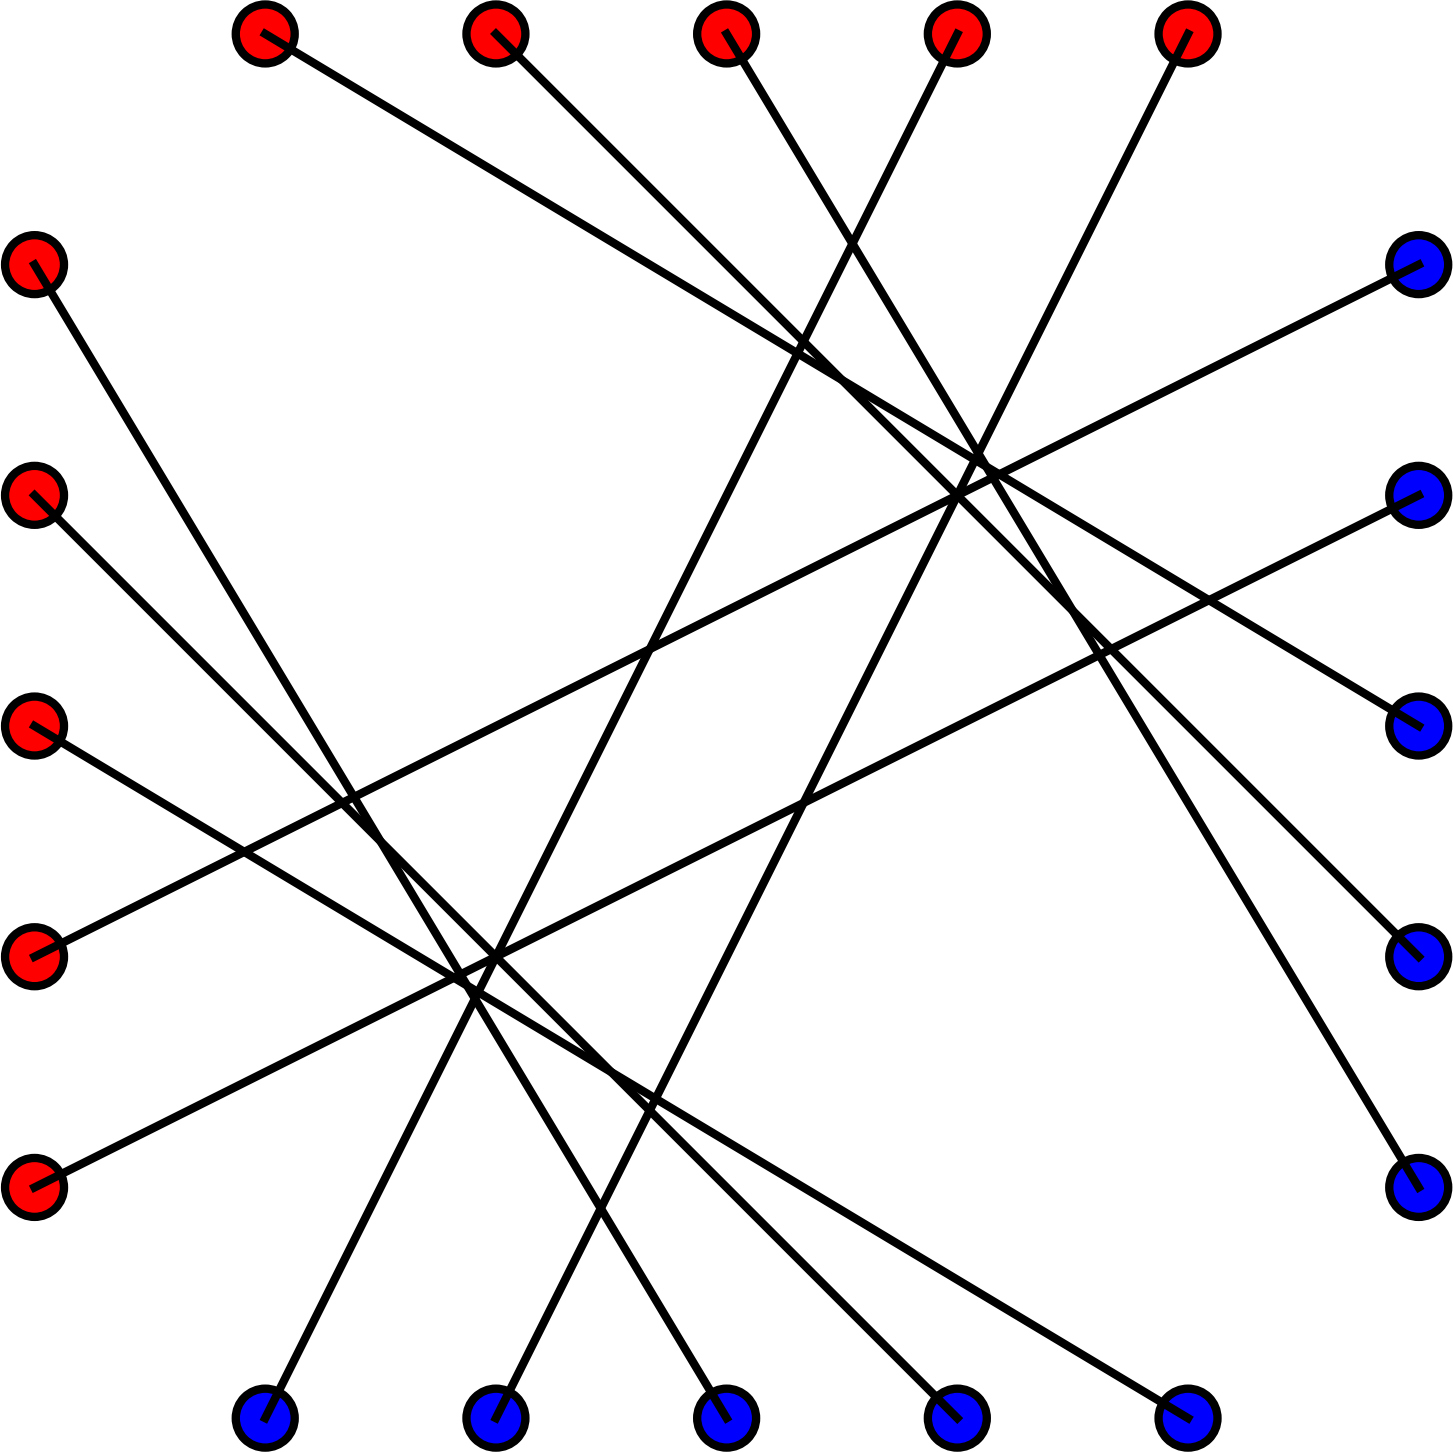
\includegraphics[width=\textwidth]{samples/1/l1_attract_coupling.png}
        \caption{$\LL_1^{-1}$, attractive cost}
    \end{subfigure}
    \caption{Various optimal coupling, depending on the associated cost matrix. }
    \label{fig:some_couplings}
\end{figure}
